\documentclass[./main.tex]{subfiles}

\begin{document}
\renewcommand{\thesubsubsection}{C\arabic{subsubsection}}

\subsection{dObtención del software de Oracle y configuración de Red}\label{sec:obtenc-del-soft}
Descargamos la base de datos de
\href{https://www.oracle.com/database/technologies/oracle-database-software-downloads.html}
{la página de descargas de Oracle} (el cual requiere registro previo), lo descargamos y lo
transferimos a la máquina virtual.
\begin{codeC}{shell-session}{Sesión de shell transfiriendo archivo}
$ scp -P 2222 Descargas/LINUX.X64_193000_db_home.zip candrade@127.0.0.1:/home/candrade/Descargas/
candrade@127.0.0.1's password:
LINUX.X64_193000_db_home.zip                                                          100% 2918MB  44.2MB/s   01:05
\end{codeC}

% $

Mientras se transfiere/descarga el software, podemos manipular la red, anteriormente se usaba una
red NAT entre la máquina anfitriona y la huésped. Ahora vamos a conectarla con un adaptador puente
en VirtualBox, en la configuración de la red en la pestaña \textit{Adaptador 1} seleccionamos
Adaptador puente y elegimos la red que esta conectada a internet, en este caso \texttt{enp3s0}\footnote{Puede
  cambiar dependiendo del estado de la máquina anfintrion}
\begin{figure}[H]
  \centering
  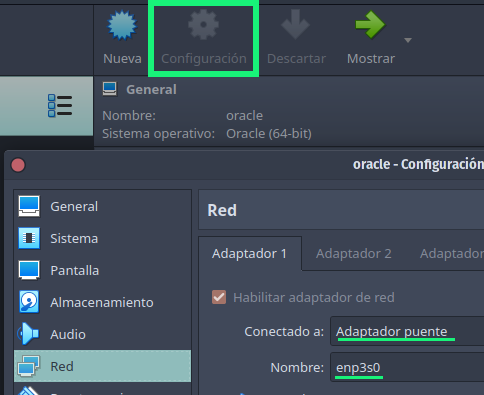
\includegraphics[width=0.8\columnwidth]{red}
  \caption{Configuración de red de la VM}\label{fig:red}
\end{figure}

Conectamos la VM a la res si se desconecto, con \texttt{ip a} en la VM
\begin{codeC}{shell-session}{Fragmento del comando \texttt{ip a} en la VM}
2: enp0s3: <BROADCAST,MULTICAST,UP,LOWER_UP> mtu 1500 qdisc fq_codel state UP group default qlen 1000
    link/ether 08:00:27:fa:6f:2e brd ff:ff:ff:ff:ff:ff
    inet 192.168.0.103/24 brd 192.168.0.255 scope global dynamic noprefixroute enp0s3
\end{codeC}

Vemos que la ip que se le asignó a nuestra VM es $192.168.0.103$, sabiendo que la máquina anfintriona
tiene la ip $192.168.0.107$, procedemos a añadir dichas máquinas en los archivos \texttt{/etc/hosts}
con sus respectivos \texttt{hostsnames}
\begin{codeCL}{bash}{Texto que se inserto en \texttt{/etc/hosts} en la MA}{src:hosts-vm}
192.168.0.103 oraclebdd oraclebdd.unam.mx
\end{codeCL}

\begin{codeCL}{bash}{Texto que se inserto en \texttt{/etc/hosts} en la VM}{src:hosts-vm}
127.0.1.1 oraclebdd oraclebdd.unam.mx

192.168.0.107 Arch-R7
\end{codeCL}


\subsubsection{Salida del Comando Ping}\label{sec:salida-del-comando}

\subsubsection{Explicación opciones -u, -g, -G}\label{sec:expl-opci-u}

\subsubsection{Salida del script de validación}\label{sec:salida-del-script}





\end{document}
